% !TEX program = XeLaTeX
% Standalone version of the onboard-algorithm block from poster.tex
% (Navigation ESKF + IPP EKF + rocket/env models).
% Output: figures/pico_architecture.pdf  — for the PICO pitch IPP slide.
\documentclass[border=10pt]{standalone}
\usepackage{fontspec}
\usepackage{xcolor}
\usepackage{tikz}
\usetikzlibrary{arrows.meta, positioning, shapes.geometric}

\setmainfont[
  Path=resources/fonts/,
  Extension=.ttf,
  BoldFont=*bd,
  ItalicFont=*i,
  BoldItalicFont=*bi
]{arial}

\definecolor{darkgray}{HTML}{232834}

\begin{document}
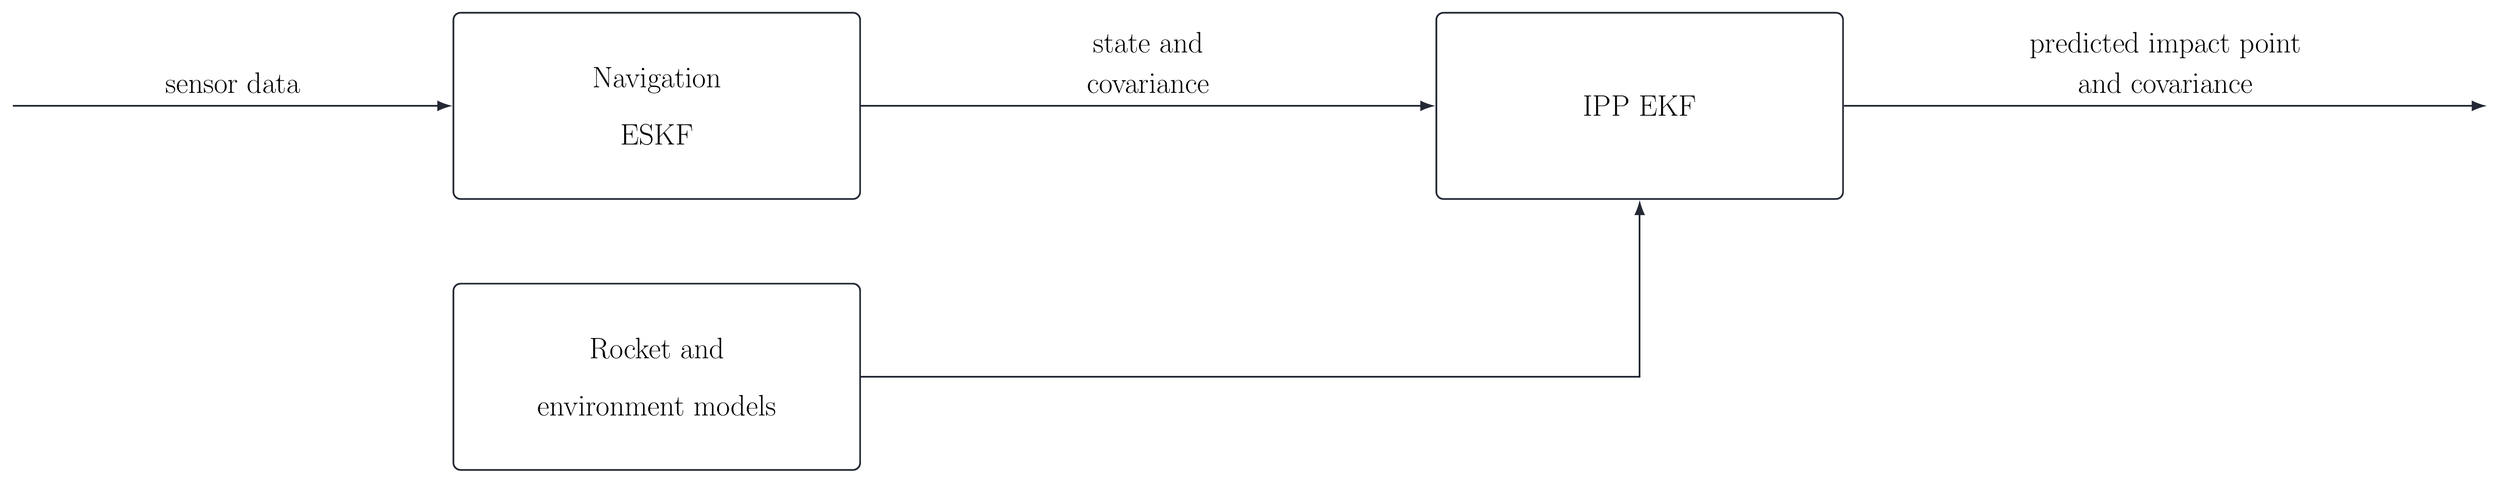
\begin{tikzpicture}[
    font=\fontsize{40}{48}\selectfont,
    box/.style={rectangle, rounded corners=6pt, draw=darkgray, line width=1.4pt,
                fill=white, align=center, minimum width=12cm, minimum height=5.5cm},
    arrow/.style={-{Latex[length=4.5mm, width=3.2mm]}, line width=1.5pt, draw=darkgray},
    flowlabel/.style={font=\fontsize{28}{34}\selectfont, align=center, fill=white,
                      inner xsep=3pt, inner ysep=2pt}
  ]
    \node[box] (nav)     at (19,0)  {Navigation\\ESKF};
    \node[box] (cartipp) at (48,0)  {IPP EKF};
    \node[box] (model)   at (19,-8) {Rocket and\\environment models};

    \draw[arrow] (0,0) -- (nav.west)
      node[midway, above=8pt, flowlabel] {sensor data};
    \draw[arrow] (nav.east) -- (cartipp.west)
      node[midway, above=8pt, flowlabel] {state and\\covariance};
    \draw[arrow] (model.east) -| (cartipp.south);
    \draw[arrow] (cartipp.east) -- (73,0)
      node[midway, above=8pt, flowlabel] {predicted impact point\\and covariance};
\end{tikzpicture}
\end{document}
